\documentclass{article}

\usepackage{authblk}
\usepackage{url}
\usepackage[square,numbers]{natbib}
\usepackage{color,amssymb,amsmath}
\usepackage{graphicx}
\usepackage[margin=1in]{geometry}
%\usepackage{graphicx}
%\SectionNumbersOn
%\AbstractOn

\title{Supplementary Information for: A Natural Representation of Functions that Facilitates 'Exact Learning'}
%\author{Benedict W. J.~Irwin}


\date{\today}
\begin{document}

%\email{ben.irwin@optibrium.com}
%\affiliation{Optibrium, F5-6 Blenheim House, Cambridge Innovation Park, Denny End Road, Cambridge, CB25 9PB, United Kingdom}
%\alsoaffiliation{Theory of Condensed Matter, Cavendish Laboratories, University of Cambridge, Cambridge, United Kingdom}

\author[1,2]{Benedict W. J.~Irwin}
\affil[1]{Theory of Condensed Matter, Cavendish Laboratories, University of Cambridge, Cambridge, United Kingdom}
\affil[2]{Optibrium, F5-6 Blenheim House, Cambridge Innovation Park, Denny End Road, Cambridge, CB25 9PB, United Kingdom}
\affil[ ]{\textit {ben.irwin@optibrium.com}}


\maketitle

\begin{abstract}
This is the supporting information for the paper "A Natural Representation of Functions that Facilitates 'Exact Learning'".
Here we discuss a few more technical ideas and extended discussion that would interrupt the flow of the main work.
\end{abstract}


\section{General Statements and Recap of the Work}
In the main text, we presented a collection of mathematical tools that have great potential to enable innovations in machine learning. We communicate a fundamental pattern across analytic functions, which often arise as solutions to problems in all domains of science. A hierarchy of functions that follow this pattern reveals the kinds of trainable parameters that would be used for a machine learning model developed in this framework. A multivariate extension is considered for each of the functions in the hierarchy and how those representations might be more convenient and interpretable for the development of machine learning algorithms. \\

In principle, this method could allow the exact learning of functional forms or statistical distributions which feature in natural problems arising in physics and mathematics using comparatively few parameters to traditional machine learning approaches. The solutions drawn from highly generalized classes of functions have been documented rigorously in the space of special functions for mathematics, but have not yet have been considered by a wide audience for the purposes of machine learning and data analysis. There is reason that any method that could connect these concepts successfully would also carry across to non-exact problems and approximate solutions for use cases in traditional machine learning settings where the desired function is an interpolation of noisy real life data.\\

For a situation where there are many inputs and many outputs for a multivariate function, the full correlated probability distribution for inputs and outputs all taking their respective values could be learned by assuming a highly generalised analytic expansion in many variables which is assumed to be described by a multivariate analogue of a highly generalised Meijer-G function, or analogous function which admits definition through a Barnes integral. The moments of the distribution of choice are extracted using the generalised Ramanujan master theorem and training is directly applied to the coefficients of the full probability distribution. The duality is manipulated through a multivariate Mellin transform which can handle the constraint of normalisation for probability distributions.


\section{Potential Limitations of the Methods}
We should quickly review the potential limitations of the method. A few technical details were glossed over in the main text for sake of clarity.
\begin{enumerate}
\item  Firstly, all the functions in the current implementation should only take values in the positive quadrant of the N-dimensional domain, i.e. $[0,\infty)^N$. This is the natural integration range on the definition of the Mellin transform. It is possible to extend the Mellin transform to the range $(-\infty,\infty)$ (Galambos \& Simonelli (2004, p. 16)) by use of the equation  $$\mathcal{M}_X(s) = \int_0^\infty  x^s dF_{X^+}(x) + \gamma\int_0^\infty x^s dF_{X^-}(x).$$ However this doubles up on the number of integrals in each dimension and in $2^N$ quadrants in multiple dimensions. Of course many functions can be written in a slightly different way to reduce the domain of inputs to $[0,\infty)$ using a composition of functions.
\item The functions must be analytic to be represented in this work. They must have a positive integer power series. There may be analogous methods available for negative integer powers and generalised series with rational or even real integer powers, but further work is required. Many functions of interest are covered in the current range.
\item The functions must be representable by the highly generalised hierarchy, essentially by the Rathie-I function or a simpler subset. Some functions have Mellin transforms or fingerprints which are not products of gamma functions and their reciprocals. For example, functions that have hypergeometric representations for their moments. It may be possible to come up with an iterated fingerprint to get round this (i.e. 'moments of moments'), but more work is required to develop this.
\item For the Meijer-G type functions and above discussed in the main text, the concept of a Mellin transform has some subtleties, although the fingerprint is still a useful concept, there can be more than one contour integration path needed for the function. Some useful ideas are developed by Peasgood \cite{Peasgood2009}.
\item Optimisation over gamma, and log-gamma functions has good sides and bad sides. The derivatives are expressible as digamma functions for example which is convenient, and in the case of log-gamma functions, there is much cancellation in the gradients which could lead to fast optimisation routines. However, it is likely that a complex number should be received as input and output. On the real line, gamma functions have poles at negative integers, and these need to be avoided by the gradient method otherwise instabilities occur. Complex gradient methods are not supported widely in major machine learning packages at the moment. There are likely other quirks to the analytic continuation side of the function definitions that need to be considered
\item The Mellin transform of a function provides not only a new 'transformed' function, but also a strip of holomorphy and it is the \emph{pair} that define the Mellin transform (to make it unique). This strip can be interpreted as the range of moments that are well defined for a given distribution, and choosing exponents $s$ in the exact learning algorithm that are outside of this range will cause problems.
\item Bias may occur in sampling the above range of exponents for distributions. For example a distribution that as infinite valid moments, will be harder to sample from, because when the machine learning is fitting the fingerprint, it should ideally be fit across all exponents $s$ that are possible, but the very large numbers will not be easy to sample.
\item Methods may need to be developed for the intepretation of the parameters fitted in fingerprints. For example where these take integer values, we need to be reasonably confident that the algorithm has converged on the integer value before rounding it to recreate a mathematical closed form.
\item There is a large permutation degeneracy in fitting some of the parameters in the fingerprint. Methods to overcome this may assist with the fitting.
\end{enumerate}


\section{Appendix 1: Examples of the Mellin Transform and RMT}
\subsection{Mellin Transform}
Mellin transforms depend strongly on the so called 'strip of holomorphy' for a given function. This is covered in detail by Geenens \cite{Geenens2017}. A comprehensive table of Mellin transforms is given by `Caltech Tables of Integral Transforms' \cite{Erdelyi1954}. We define the Mellin transform as an integral transform of a function $f(x)$ as
\begin{equation}
\mathcal{M}[f(x)](s) = \int_0^\infty x^{s-1}f(x) dx = \varphi(s)
\end{equation}
which will obviously only converge for certain choices of functions $f(x)$ and certain exponents $s$. The set of complex values $s$ that converge for a function $f$ is the so called strip of holomorphy. It should be noted that if $f(x)$ is a probability distribution with positive semi-infinite support, through the definition of the Mellin transform we must have $\varphi(1)=1$ due to the normalisation constraint \cite{Geenens2017}. This concept will be used later to automatically train functions which can act as probability distributions. The inverse Mellin transform is given by
\begin{equation}
\mathcal{M}^{-1}[\varphi(s)](x) = \frac{1}{2 \pi i}\int_{c- i \infty}^{c + i \infty} x^{-s} \varphi(s) \; ds = f(x)
\label{eqn:InverseMT}
\end{equation}
where $i$ is the imaginary unit and the limits on the integral are to be interpreted as a line in the imaginary axis passing through a real constant $c$ which must lie in the strip of holomorphy and not cross the poles in the function $\varphi(s)$. To avoid the complexity of such inverse transforms we use the Ramanujan master theorem (RMT) as a bridge to convert between a function $f(x)$ and its Mellin transform $\varphi(s)$.


\subsubsection{Negative Exponential}
One of the simplest functions to use as an example is $f(x)=e^{-x}$, the Mellin transform of this is
\begin{equation}
\mathcal{M}[e^{-x}](s) = \int_0^\infty x^{s-1}e^{-x} \; dx = \Gamma(s)
\end{equation}
which can be seen to be an integral definition of the Euler gamma function. If we look at the series expansion of $e^{-x}$ we have
\begin{equation}
e^{-x} = \sum_{k=0}^\infty \frac{(-1)^k}{k!} x^k = \sum_{k=0}^\infty \chi_k \phi(k) x^k
\end{equation}
here we see that the coefficient function $\phi(k)$ is always $1$. Which by the RMT predicts the Mellin transform of $e^{-x}$ to be
\begin{equation}
\mathcal{M}[e^{-x}](s) = \Gamma(s)\phi(-s) = \Gamma(s)\cdot 1 = \Gamma(s)
\end{equation}
which is in agreement with the integral definition.
\subsubsection{Binomial $(1+x)^{-1}$}
We can consider the function $f(x) = \frac{1}{1+x}$ with expansion
\begin{equation}
\frac{1}{1+x} = \sum_{k=0}^\infty \frac{(-1)^k}{k!} k! x^k = \sum_{k=0}^\infty \chi_k \Gamma(k+1) x^k
\end{equation}
here the continuation of the coefficient function $\phi(k) = \Gamma(k+1)$. We can use the RMT to predict that the Mellin transform is
\begin{equation}
\mathcal{M}\left[\frac{1}{1+x}\right](s) = \Gamma(s)\phi(-s) = \Gamma(s)\Gamma(1-s)
\end{equation}
if we evaluate the integral directly this is the case.
\subsubsection{Binomial $(1+x)^{-a}$}
As before we write the series expansion
\begin{equation}
\frac{1}{(1+x)^a} = \sum_{k=0}^\infty \binom{-a}{k} x^k = \sum_{k=0}^\infty \chi_k \frac{\Gamma(k+a)}{\Gamma(a)} x^k
\end{equation}
Then the Mellin transform by the RMT is 
\begin{equation}
\mathcal{M}\left[\frac{1}{(1+x)^a}\right](s) = \frac{\Gamma(s)\Gamma(a-s)}{\Gamma(a)}
\end{equation}


\section{What Problems Could be Solved?}
Here we will discuss the types of problems that are interesting to solve using the exact learning concept. Obviously anything that creates a high precision probability distribution as output will be reasonably well behaved. 
\begin{enumerate}
\item Consider solutions to differential equations, for example the Schr\"odinger equation. We could define a potential, solve the time-independent equation for a density (there are many methods for this), then this high resolution density could be checked using exact learning to see if a closed form, or analytic solution exists.
\item Perhaps a Monte-Carlo type simulation of a distribution, if there was enough data.
\item An integral convolution of two distributions that is hard to solve. These might arise in statistics. Examples might be the distributions of eigenvalues of matrices drawn from distributions in problems similar to random matrix theory. \\
\item High dimensional equations that are hard to visualise.
\item Finding the expansion coefficients of compositions of functions
\item Finding the expansion coefficients of inverses of functions using series reversion.
\item Finding a closed form for a function which is in principle not complicated, but is laborious to calculate due to the length of the equations. For example a function of a molecule, which might require a tedious calculation for every atom and bond, but the solution will be a simple, but large combination of many terms.
\item Some form of generalisation where instead of generating functions (i.e. series expansions), we have generating functionals.
\end{enumerate}

If these are not directly applicable, then extensions to the framework to work towards these goals may be fruitful. \\

With the power of modern numerical integration methods, exact learning might be useful to evaluate integrals which cannot be resolved in a closed form analytically. Take for example the integral:
\begin{equation}
I(a,b,c) = \int_0^1 \frac{dx}{\sqrt[3]{a x + b x^2 + cx^3}}
\end{equation}
which would be tricky to evaluate. We can measure this to high precision numerically for a range of  values of $a,b,c$. And from this we measure the variation of the solution with respect to each parameter to determine whether a closed form exists. We'll briefly cover the idea of variation of solution.

\subsection{Variation of Solution} 
Some problems have additional input parameters to the problem, $\alpha$, such that when $\alpha$ is varied the resulting distribution or function changes. We can consider the various outputs with exact learning, and additionally vary the parameter $\alpha$ to the problem and look at the changes in the solution. The gradients will help us numerically identify cases where parameters have certain relations. The fingerprint of a function is $\mathcal{M}[f(x)](s,\cdots)$, where $\cdots$ are additional parameters of the problem. Then we may see the following condition arise:
\begin{equation}
\frac{\partial}{\partial \alpha} \log \mathcal{M}[f](s,\alpha) = \frac{1}{\mathcal{M}[f](s,\alpha)}\frac{\partial}{\partial \alpha} \mathcal{M}[f](s,\alpha) \approx A\frac{s}{\alpha}.
\end{equation}
(Note that the majority of the fingerprint which does not depend on $\alpha$ will cancel out). Here we can identify that $\alpha$ is a simple scale factor on the final solution. If we instead observe 
\begin{equation}
\frac{\partial}{\partial \alpha} \log \mathcal{M}[f](s,\alpha) \approx \psi^{(0)}(a+s) - \psi^{(0)}(s)
\end{equation}
then there is a scaling factor term on the fingerprint of the form
\begin{equation}
\frac{\Gamma(\alpha+s)}{\Gamma(\alpha)},
\end{equation}
which is not uncommon, as these look like normalising terms for distributions. Because of the regularity of the structure of fingerprints, it will be fairly easy to identify a few common cases, which will allow us to understand how external parameters are best represented in the fingerprint.

\subsection{List of Representable Functions}
Here we list some (but by no means all) of the functions which can be expressed by the highly generalised forms discussed in the main work. Table \ref{tab:hyp} shows the functions that can be expressed using generalised hypergeometric series along with extra pre-factors factors (usually gamma, Pochhammer or simple power functions, which are compatible with the exact learning algorithm described in the main work).

\begin{table}[h]
\centering
\begin{tabular}{|p{4.5cm}|p{1.5cm}|p{5cm}|}
\hline
Hypergeometric \newline Representation & Common \newline Expression & Name\\
\hline
$_0F_0(;;z)$&$e^z$ & Exponential Function\\
$_1F_0(a;;z)$ & $(1-z)^{-a}$ & Binomial\\
$\frac{(\frac{x}{2})^\alpha}{\Gamma(\alpha+1)} _0F_1(;\alpha+1;\frac{-x^2}{4}) $ & $J_\alpha(x)$ & Bessel (1) \\
$\frac{(\frac{x}{2})^\alpha}{\Gamma(\alpha+1)} _0F_1(;\alpha+1;\frac{x^2}{4}) $ & $I_\alpha(x)$ & (modified) Bessel (1) \\
$_1F_1(a;b;z)$ & $M(a,b,z)$ & Confluent Hypergeometric \newline Function I (Kummer) \\
$\frac{2 z}{\sqrt{\pi}}\;_1 F_1(\frac{1}{2};\frac{3}{2};-z^2)$ & $\mathrm{erf}(z)$ & Error Function \\
$\frac{x^a}{a}\;_1F_1(a;1+a;-x)$ & $\gamma(a,x)$ & (Lower) Incomplete Gamma Function\\
$\frac{(\alpha+1)_n}{n!} \;_1F_1(-n;\alpha+1;z)$ & $L(n,\alpha,z)$ & (Generalized) Laguerre \newline Polynomials \\
$(2z)^n \;_2F_0(-\frac{n}{2},\frac{(1-n)}{2};;-z^{-2})$ & $H_n(z)$ & Hermite Polynomials\\
$z^{-a} _2F_0(a,1+a-b;;-z^{-1})$ & $U(a,b,z)$ & Confluent Hypergeometric \newline Function II (Tricomi) \\
$_2F_1(-n,n+1;1;\frac{(1-x)}{2})$ & $P_n(x)$ & Legendre Polynomials\\
$(\cdots)\;_2F_1(\cdots)$ & $C^{(\lambda)}_n(x)$ & Gegenbauer Polynomial\\
$(\cdots)\;_2F_1(\cdots)$ & $P^{(\alpha,\beta)}_n(x)$ & Jacobi Polynomial\\
$(\cdots)\;_2F_1(\cdots)$ & $R^m_n(x)$ & Zernike Polynomial \\
$(\cdots)\;_2F_1(\cdots)$ & $\cdots$ & Spherical Harmonics \\
$ \frac{z^a}{a} _2F_1(a,1-b;a+1;z)$  & $B(z,a,b)$ & Generalised Beta Function \\
$_2F_0()$ & $Ei(z)$ & Exponential Integral \\
$\left(\frac{z}{2}\right)^n\;_3F_0(-n,\frac{1-n}{2},\frac{2-n}{2};;-\frac{4}{z^2})$ & $s_n(z)$ & Mott Polynomials \\
$x_3F_2(1,1,1;2,2;x)$ & $\mathrm{Li}_2(x)$ & Dilogarithm \\
$(\cdots)\;_3F_2(\cdots)$ & $\cdots$ & Clebsch-Gordan coefficients \\
$(\cdots)\;_1F_q(\cdots)$ & $\cdots$ & Generalized Mittag-Leffler \\
\hline
\end{tabular}
\caption{Some examples of hypergeometric representations of common (and not so common) functions. Some of these are very general polynomials already that cover others as special cases. Sometimes the full formula is omitted to save space, but the order of hypergeometric function required is retained.}
\label{tab:hyp}
\end{table}

\subsection{Meijer-G Represents Even More Functions}
Simple functions expressible by the Meijer-G function include sin, cos, sinh, cosh, arcsin, arctan, arccot, $log(1+x)$, Heaviside theta (step functions), the upper and lower incomplete gamma functions $\Gamma(\alpha,x)$ and $\gamma(\alpha,x)$, and their $\alpha$-derivatives (Wikipedia has information on this for example). More advanced functions include: all Bessel functions of the first and second kind and their modified forms, $J_\nu(x)$, $Y_\nu(x)$, $I_\nu(x)$, $K_\nu(x)$, the Lerch transcendent $\Phi(x,n,a)$, and therefore the Hurwitz zeta function, Polylogarithm $\mathrm{Li}_s(z)$, Riemann zeta function, Dirichlet eta function and Legendre chi function.

\section{Examples}
Here we have a few examples that show a basic fitting method.

\subsection{A Numeric Test : 1D- Exponential}
We generated $1000$ samples from the distribution $x_1 \sim \exp(-x)$ and attempted to fit to $\phi(s) = \frac{\Gamma(b + a s)}{\Gamma(b)}$. The algorithm ran till it converged. The final parameters were $a = [0.00132615]\approx 0$ and $b=[1.0014696]\approx 1$. In 1-D we may approximate this as \begin{equation}
\tilde{F}^{(1)}(1;;0,;x) = \sum_{k=0}^\infty \frac{(-1)^k}{k!} \frac{\Gamma(1+0k)}{\Gamma(1)} x^k = e^{-x}
\end{equation}
the original distribution is recreated for this extremely simple case.


\subsection{Complex Fitting}
For a known p.d.f of a folded Gaussian with unit variance, we sample $100000$ points and define a fingerprint as
\begin{equation}
\phi(s) = \alpha \beta^s \Gamma(\gamma s).
\end{equation}
We use this to give an example of complex fitting. We sample a range of $400$ exponents $s$ which are complex numbers with real parts uniformly sampled from $1$ to $7$ and imaginary parts uniformly sampled from $-4$ to $4$. We then calculate the expected value of the samples for each exponent $s_k$ in the sample as 
$$
E[x^{s_k-1}] = \frac{1}{N}\sum_j x_j^{s_k-1}
$$
From this we use a BFGS minimiser to minimise:
\begin{equation}
L = \sum_k (Re[\log\phi(s)]-Re[\log E[x^{s_k-1}]])^2 + \min_{\tau \in \{-1,0,1\}}(Im[\log\phi(s)]+2\tau \pi -Im[\log E[x^{s_k-1}]])^2,
\end{equation}
as a function of parameters $[\alpha,\beta,\gamma]$, who converge on the values [0.39397852931,1.41650198672,0.49494035]. Plots of the converged parts are given in figures \ref{fig:A} and \ref{fig:B}. The points overlap almost perfectly. In the imaginary alignment, a small cluster of points are exactly $2 \pi$ away from their correct value, due to a branch cut in the complex log and log gamma functions used for the fitting. We adapted the loss function to account for this, taking the minimum difference of three possible neighbouring branches.\\


\begin{figure}[h!]
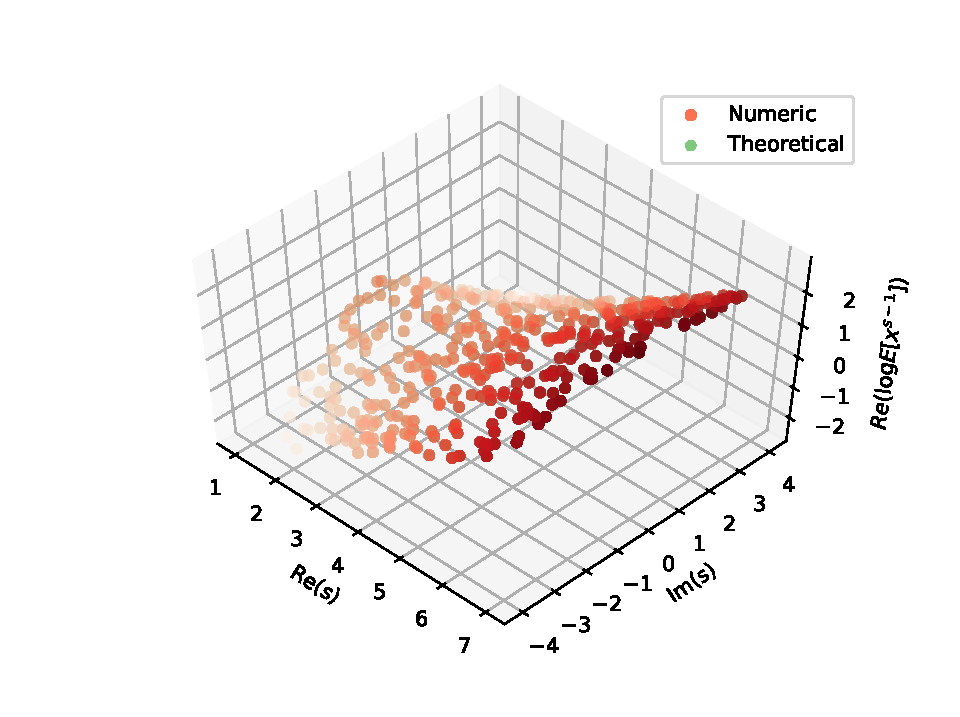
\includegraphics[scale=1]{Re_Fit_Final}
\caption{The real part of the log moments fitted to the log theoretical fingerprint}
\label{fig:A}
\end{figure}

\begin{figure}[h!]
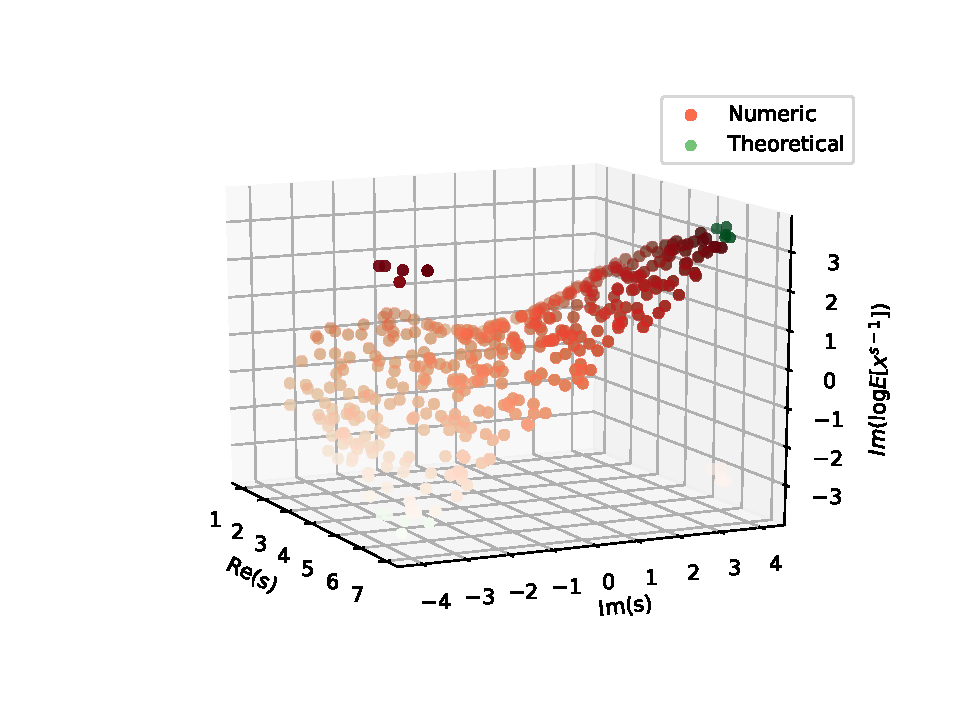
\includegraphics[scale=1]{Im_Fit_Final}
\caption{The imaginary part of the log moments fitted to the log theoretical fingerprint}
\label{fig:B}
\end{figure}

If we somehow recognise or interpret the parameters as $\beta \approx \sqrt{2}$, $\gamma \approx 0.5$, we get
$$
\phi^*(s) = \alpha \sqrt{2}^s \Gamma\left(\frac{s}{2}\right).
$$
We analytically find that the inverse Mellin transform is
$$
\mathcal{M}^{-1}[\phi^*(s)](x) = 2ae^{-x^2/2}
$$
which is the correct form as the original distribution. In practice recognising the coefficients may be hard and future development is going to be required to identify integers, rational and special constants. The algorithm may need to be repeated with different initial conditions to get a distribution of values for each parameter and to hone in on likely values and use statistical tests.\\

\section{Walkthrough of GRMT on Generalised Probability Distribution}
Suppose we have a distribution $P(\mathbf{x})$ with multivariate $\mathbf{x}$. Suppose these inputs all in the positive real numbers. The fundamental assumption behind the GRMT is to assume a multivariate analytic expansion of this distribution in terms of a set of coefficients $\varphi$. Assume a form for the multivariate distribution, using a vector index notation $\mathbf{k} = (k_1, \cdots, k_n)$ where the sum extends from $0$ to $\infty$ for each index
\begin{equation}
P(\mathbf{x}) = \sum_{\mathbf{k}=0}^\infty  \chi(\mathbf{k})\varphi(\mathbf{k})\mathbf{x}^{\mathbf{A}\mathbf{k}+\mathbf{b}}_\Pi
\end{equation}
where the $\mathbf{a}_l$ are row vectors of a matrix $\mathbf{A}$ whose coefficients describe the relationship between the variables $\mathbf{x}$ and the summation indices $\mathbf{k}$, the $b_l \in \mathbf{b}$ are constant terms in the exponents of the variables, $f(\mathbf{k})$ is a multivariate coefficient function which defines the moments of the probability distribution. We may write the expectation of a given multivariate moment as a function of the vector of exponents of the variables $\mathbf{s}$
$$
\mathcal{E}_P(\mathbf{s}) = \mathbb{E}\left[\prod_{k=0}^n X_k^{s_k-1}\right] =\int_{[0,\infty)^{n}} \mathbf{x}_\Pi^{\mathbf{s}-\mathbf{1}} P(\mathbf{x}) \; d \mathbf{x}
$$
where the $\mathbf{s}-\mathbf{1}$ has been included to make the expression match the definition of a multivariate Mellin transform. As a consequence by the GRMT this is representable in terms of the divergent bracket symbols of [Gonzalez et. al] \citep{Gonzalez2015}, which they define as
\begin{equation}
\langle s \rangle = \int_0^\infty x^{s-1} \; dx
\end{equation}
which are used to \emph{formally} manipulate the series expansion according to their rules. Note that due to separability the integral of a product of variables to exponents is simply a product of bracket symbols
\begin{equation}
\int_{[0,\infty)^n} \mathbf{x}^{\mathbf{s-1}}_\Pi\;d \mathbf{x} = \prod_{l=1}^n \int_0^\infty x_l^{s_l-1} \; dx_l = \prod_{l=1}^n \langle s_l \rangle
\label{eqn:bracket}
\end{equation} 


We may write explicitly using vector arguments for brevity
\begin{equation}
\mathcal{M}_P(\mathbf{s}) = \int_{[0,\infty)^{n}} \mathbf{x}^{\mathbf{s-1}} \sum_{\mathbf{k}=0}^\infty  \chi(\mathbf{k})\varphi(\mathbf{k}) \mathbf{x}^{\mathbf{A}\mathbf{k}+\mathbf{b}}_\Pi \; d \mathbf{x}
\end{equation}
under linearity bring the product of variables under the summation sign and combine it with the variables being summed over
\begin{equation}
\mathcal{M}_P(\mathbf{s}) = \int_{[0,\infty)^{n}} \sum_{\mathbf{k}=0}^\infty  \chi(\mathbf{k})\varphi(\mathbf{k}) \mathbf{x}^{\mathbf{s-1}}_\Pi \mathbf{x}^{\mathbf{A}\mathbf{k}+\mathbf{b}}_\Pi \; d \mathbf{x}
\end{equation}
\begin{equation}
\mathcal{M}_P(\mathbf{s}) = \int_{[0,\infty)^{n}} \sum_{\mathbf{k}=0}^\infty  \chi(\mathbf{k})\varphi(\mathbf{k})\mathbf{x}^{\mathbf{A}\mathbf{k}+\mathbf{b}+\mathbf{s-1}}_\Pi \; d \mathbf{x}
\end{equation}
swapping the sum and the integral under linearity would give
\begin{equation}
\mathcal{M}_P(\mathbf{s}) = \sum_{\mathbf{k}=0}^\infty  \chi(\mathbf{k})\varphi(\mathbf{k})\int_{[0,\infty)^{n}} \mathbf{x}^{\mathbf{A}\mathbf{k}+\mathbf{b}+\mathbf{s-1}}_\Pi \; d \mathbf{x}
\end{equation}
using equation \ref{eqn:bracket} we can convert these to divergent bracket symbols
\begin{equation}
\mathcal{M}_P(\mathbf{s}) = \sum_{\mathbf{k}=0}^\infty  \chi(\mathbf{k})\varphi(\mathbf{k}) \prod_{l=1}^n \langle \mathbf{a}_l \cdot \mathbf{k} + \mathbf{b} + \mathbf{s} \rangle
\end{equation}
according to rule 2 of the method of bracket from Gonzalez et al. \cite{Gonzalez2015} - which says that the contents of each divergent bracket symbol must vanish to keep the result convergent - this summation can be written by the generalised Ramanujan master theorem as 
\begin{equation}
\mathcal{M}_P(\mathbf{s}) = \frac{\varphi(\mathbf{k}^*) \prod_{l=0}^n \Gamma(-k_l^*)}{|\det(\mathbf{A})|}
\end{equation}
for $k^*_m$ as the values that satisfy the linear system of equations by vanishing the set of $\langle \cdot \rangle$ brackets. That is the solution to \begin{equation}
\mathbf{A}\mathbf{k}^*+\mathbf{b}+\mathbf{s} = \mathbf{0}
\end{equation} 


\section{Multidimensional Generalised Functions}
Here we give a few examples of working with multivariate functions.

\subsection{Appell $F_1$ Function}
This can be written as a double contour integral
\begin{equation}
F_1(a;b_1,b_2;c;z_1,z_2) = \frac{1}{(2\pi i)^2}\int_{L^*} \int_L  \bar{\phi}(s,t) (-z_1)^{-s_1}(-z_2)^{-s_2} ds_1 ds_2
\end{equation}
with \begin{equation}
\bar{\phi}(s_1,s_2) = \frac{\Gamma(c)\Gamma(a-s_1-s_2)\Gamma(b_1-s_1)\Gamma(b_2-s_2)\Gamma(s_1)\Gamma(s_2)}{\Gamma(a)\Gamma(b_1)\Gamma(b_2)\Gamma(c-s_1-s_2)}
\end{equation}
Which some parts can be rewritten as 
\begin{equation}
\bar{\phi}(s_1,s_2) = \frac{\Xi[c])\Xi[a-\mathbf{1}\cdot\mathbf{s}]\Xi[\mathbf{b}-\mathbf{s}]\Xi[\mathbf{s}]}{\Xi[a]\Xi[\mathbf{b}]\Xi[c-\mathbf{1}\cdot\mathbf{s}]}
\end{equation}
the function is defined with $\mathbf{M}=\mathbf{I}_2$ which has determinant $1$. Because of this we know that $\mathbf{k}^* = -\mathbf{s}$, this explains the $\Xi[\mathbf{s}]$ term.

\subsubsection{Gauss Hypergeometric to Lauricella Function in N-D}
There are four Lauricella functions in $D$ dimensions. The function of type-A for example is
\begin{equation}
F_A^{(n)}(a, b_1,\ldots,b_n, c_1,\ldots,c_n; x_1,\ldots,x_n) = 
\sum_{i_1,\ldots,i_n=0}^{\infty} \frac{(a)_{i_1+\ldots+i_n} (b_1)_{i_1} \cdots (b_n)_{i_n}} {(c_1)_{i_1} \cdots (c_n)_{i_n} \,i_1! \cdots \,i_n!} \,x_1^{i_1} \cdots x_n^{i_n}
\end{equation}
One can conceive a higher generalisation of this which should be one of the most general (at the expense of additional parameters). Define
\begin{equation}
\tilde{F}^{D}(\mathbf{a};\mathbf{b};\mathbf{V,W};-\boldsymbol\eta \odot\mathbf{x}) = \sum_{\mathbf{k}} \chi(\mathbf{k})\frac{\prod_{j=1}^D (a_j)_{\mathbf{v}_j \cdot \mathbf{k}}}{\prod_{j=1}^D (b_j)_{\mathbf{w}_j \cdot \mathbf{k}}} \boldsymbol\eta^{\mathbf{k}}_\Pi\mathbf{x}^{\mathbf{k}}_\Pi
\end{equation}
which in terms of gamma functions is 
\begin{equation}
\tilde{F}^{D}(\mathbf{a};\mathbf{b};\mathbf{V,W};-\boldsymbol\eta \cdot\mathbf{x}) = \sum_{\mathbf{k}} \chi(\mathbf{k})\frac{\prod_{j=1}^D \Gamma(b_j)\Gamma(a_j + \mathbf{v}_j\cdot \mathbf{k})}{\prod_{j=1}^D \Gamma(a_j)\Gamma(b_j+\mathbf{w}_j\cdot \mathbf{k})} \boldsymbol\eta_\Pi^\mathbf{k}\mathbf{x}_\Pi^\mathbf{k}
\end{equation}
which in terms of $\Xi$ is
\begin{equation}
\tilde{F}^{D}(\mathbf{a};\mathbf{b};\mathbf{V,W};-\boldsymbol\eta \cdot\mathbf{x}) = \sum_{\mathbf{k}} \chi(\mathbf{k})\frac{\Xi[\mathbf{b}]\Xi[\mathbf{a}+\mathbf{Vk}]}{\Xi[\mathbf{a}]\Xi[\mathbf{b+Wk}]} \boldsymbol\eta_\Pi^\mathbf{k}\mathbf{x}_\Pi^\mathbf{k}
\end{equation}
because $\mathbf{M}=\mathbf{I}_D$ by the GRMT the Mellin transform is equal to \begin{equation}
\mathcal{M}[\tilde{F}^{D}(\mathbf{a};\mathbf{b};\mathbf{V,W};-\boldsymbol\eta \cdot\mathbf{x})](s) = \frac{\Xi[\mathbf{b}]\Xi[\mathbf{a}-\mathbf{Vs}]}{\Xi[\mathbf{a}]\Xi[\mathbf{b-Ws}]}\Xi[\mathbf{s}]\boldsymbol\eta_\Pi^{-\mathbf{s}}
\end{equation}
in this way there is no need for a determinant which is an obstruction to training. From this standpoint the original series is reclaimable.

\subsubsection{Note:}
We do not apply the transformation rule $\Gamma(a+k) \to \Xi[\mathbf{a} + \mathbf{Mk}]$ because upon solving the GMRT we find the Mellin transform contains terms such as $\Xi[\mathbf{a} + \mathbf{Mk^*}]$ which is equal to $\Xi[\mathbf{a} - \mathbf{s}]$ by the definition of $\mathbf{k}^*$. The resulting Mellin transform is separable in terms of the elements of $\mathbf{s}$ which shows the resulting distribution is a product of marginal distributions i.e. uncorrelated random variables, which is not ideal for machine learning. If $\mathbf{M}=\mathbf{I}_D$ then the distribution is separable.


\subsubsection{Multivariate Hypergeometric Function}
Here we perform the above prescription to convert the hypergeometric function to the multivariate hypergeometric function. We have the one dimensional hypergeometric function.
\begin{equation}
_2F_1(a,b;c;-\eta x) = \sum_{k=0}^\infty \chi_k \frac{\Gamma(c)\Gamma(a+k)\Gamma(b+k)}{\Gamma(a)\Gamma(b)\Gamma(c+k)} (\eta x)^k
\end{equation}
For the higher dimensional versions we write the equivalent definition
\begin{equation}
_2\mathbf{F}_1(\mathbf{a},\mathbf{b};\mathbf{c};-\boldsymbol\eta\odot\mathbf{x}) = \sum_{\mathbf{k}}\chi(\mathbf{k})\frac{\Xi[\mathbf{c}]\Xi[\mathbf{a}+\mathbf{k}]\Xi[\mathbf{b}+\mathbf{k}]}{\Xi[\mathbf{a}]\Xi[\mathbf{b}]\Xi[\mathbf{c}+\mathbf{k}]}{(\boldsymbol\eta\odot\mathbf{x})}^{\mathbf{M}\mathbf{k}}_\Pi
\end{equation}
with the Hadamard product $\odot$. From the GRMT we know the generalised Mellin transform of this multidimensional analogue to the hypergeometric function is equal to
\begin{equation}
\int_{[0,\infty)^n}\mathrm{x}^{\mathbf{s-1}}_\Pi\;_2\mathbf{F}_1(\mathbf{a},\mathbf{b};\mathbf{c};-\mathbf{x})\; d\mathbf{x} = \frac{\phi(\mathbf{k}^*)\Xi[-\mathbf{k}^*]}{|\det(\mathbf{M})|}
\end{equation}
which is
\begin{equation}
\mathcal{M}_D[_2\mathbf{F}_1(\mathbf{a},\mathbf{b};\mathbf{c};-\mathbf{x})] = \frac{\Xi[\mathbf{c}]\Xi[\mathbf{a}+\mathbf{k}^*]\Xi[\mathbf{b}+\mathbf{k}^*]\Xi[-\mathbf{k}^*]}{\Xi[\mathbf{a}]\Xi[\mathbf{b}]\Xi[\mathbf{c}+\mathbf{k}^*]|\det(\mathbf{M})|}
\end{equation}
where $k^* = -\mathbf{M}^{-1}\mathbf{s}$.










\bibliography{bibliography}{}
\bibliographystyle{plain}


\end{document}